\addcontentsline{toc}{section}{Introduction}
\section*{Introduction}

Ce chapitre présente l'analyse des besoins et des contraintes, la conception de la solution ainsi que les choix techniques retenus pour le développement de la plateforme \textit{Numeris229}. Il expose les besoins fonctionnels et non fonctionnels du système, l'architecture générale de la solution, les spécifications conceptuelles au travers des diagrammes UML, ainsi que les choix technologiques justifiés par les impératifs de rigueur juridique, de performance et de souveraineté des données.

% ==========================================================
\section{Analyse des besoins et des contraintes}

\subsection{Besoins fonctionnels}

Les besoins fonctionnels décrivent l'ensemble des services et fonctionnalités que la plateforme \textit{Numeris229} doit fournir afin de faciliter la compréhension, l'accès et l'application du Code du Numérique de la République du Bénin (Loi N° 2017-20 modifiée par la Loi N° 2020-35).

Le système doit permettre :

\begin{itemize}
    \item de collecter, structurer et indexer l'intégralité du corpus juridique officiel du Code du Numérique (Livre Préliminaire et Livres I à VI, soit plus de 600 articles) ;
    
    \item de proposer un explorateur interactif permettant de parcourir, rechercher par mot-clé et filtrer les articles par livre, chapitre ou référence légale ;
    
    \item d'interagir avec les utilisateurs à travers un assistant conversationnel juridique en langage naturel fondé sur une architecture RAG (Retrieval-Augmented Generation) rigoureuse et exempte d'hallucinations ;
    
    \item de détecter automatiquement les questions ciblant un numéro d'article spécifique (ex. « article 55 », « art. 125 ») afin d'assurer une extraction prioritaire et exhaustive du texte légal ;
    
    \item d'effectuer une recherche documentaire hybride combinant recherche sémantique vectorielle (dense) et recherche par mots-clés exacts (sparse TF-IDF) pour garantir une couverture exhaustive des notions juridiques ;
    
    \item de ré-ordonner sémantiquement les articles candidats au moyen d'un modèle de reranking par cross-encoder afin de sélectionner les dispositions légales les plus pertinentes ;
    
    \item de générer des réponses synthétiques, fiables et expressément sourcées, citant obligatoirement le numéro de l'article et le livre concerné ;
    
    \item d'assurer un mécanisme de secours (fallback) restituant fidèlement le texte officiel de loi en cas d'indisponibilité momentanée du service de génération ;
    
    \item d'assurer la gestion complète des conversations (création, historisation, génération automatique du titre, renommage et suppression) dans un espace sécurisé dédié à l'utilisateur ;
    
    \item de gérer l'authentification et le profil des utilisateurs (inscription, connexion sécurisée par jeton, mise à jour des informations personnelles et réinitialisation de mot de passe) ;
    
    \item de garantir l'exercice effectif du droit à l'effacement en permettant la suppression intégrale et définitive du compte utilisateur et de ses historiques.
\end{itemize}

\subsection{Besoins non fonctionnels}

Les besoins non fonctionnels définissent les critères de qualité, de sécurité et d'ergonomie indispensables au bon fonctionnement d'une plateforme d'assistance juridique :

\begin{itemize}
    \item \textbf{Exactitude et fidélité juridique :} élimination stricte des hallucinations grâce à l'ancrage exclusif des réponses dans les textes de loi officiels et à la citation systématique des sources applicables ;
    
    \item \textbf{Sécurité et confidentialité des données :} protection des échanges et des données d'identification conformément aux exigences du Livre V du Code du Numérique et aux recommandations de l'APDP (Autorité de Protection des Données Personnelles du Bénin), avec chiffrement des mots de passe par salage fort (bcrypt) et isolation des sessions ;
    
    \item \textbf{Performance et temps de réponse :} réactivité de l'API REST lors de l'exécution du pipeline RAG grâce à l'indexation matricielle locale des embeddings et au découpage optimisé des contextes ;
    
    \item \textbf{Disponibilité et résilience :} continuité du service assurée par un mode dégradé fluide qui garantit la restitution des articles même lors d'une défaillance du modèle d'inférence ;
    
    \item \textbf{Ergonomie et accessibilité :} interface utilisateur moderne, réactive, dotée d'une prise en charge native des modes clair et sombre, optimisée aussi bien sur ordinateur que sur smartphone ;
    
    \item \textbf{Modularité et maintenabilité :} découpage clair entre les couches de présentation, de traitement d'API et d'intelligence artificielle afin de faciliter l'ajout ultérieur de nouvelles jurisprudences ou décrets d'application.
\end{itemize}

\subsection{Critères d'évaluation}

L'évaluation de l'efficacité et de la précision du système \textit{Numeris229} repose sur les critères suivants :

\begin{itemize}
    \item le taux de précision de l'identification des articles de loi applicables à une requête donnée ;
    
    \item la conformité et la véracité des références légales citées dans les réponses du chatbot ;
    
    \item la réduction effective du taux d'hallucination par rapport à un grand modèle de langage utilisé sans contexte documentaire ;
    
    \item le temps moyen d'exécution du pipeline RAG complet (recherche hybride, reranking et génération) ;
    
    \item la rapidité de chargement et de filtrage au sein de l'explorateur du Code du Numérique ;
    
    \item le taux de réussite des scénarios de test fonctionnels (authentification, gestion des fils de consultation, réinitialisation de mot de passe).
\end{itemize}

\subsection{Contraintes techniques}

Le développement de \textit{Numeris229} est encadré par plusieurs contraintes techniques majeures :

\begin{itemize}
    \item \textbf{Spécificité du vocabulaire juridique béninois :} nécessité d'exploiter un modèle d'embedding adapté à la langue française et au domaine juridique afin de capter la sémantique propre aux textes de loi ;
    
    \item \textbf{Structure hiérarchique complexe de la loi :} découpage rigoureux des 7 Livres en fragments (chunks) préservant le contexte hiérarchique (Livre, Titre, Chapitre, Numéro d'article) sans tronquer les dispositions normatives ;
    
    \item \textbf{Contraintes de souveraineté et d'exécution locale :} déploiement local du modèle d'inférence (LLM) sous Ollama pour préserver la confidentialité des requêtes des usagers et limiter la dépendance envers des API propriétaires tierces ;
    
    \item \textbf{Compatibilité logicielle :} interopérabilité sans couture entre le serveur backend Python (FastAPI) et l'interface utilisateur web développée sous Next.js 14 ;
    
    \item \textbf{Conformité réglementaire :} respect strict des obligations de recueil de consentement et de transparence prescrites par la législation nationale sur la protection des données personnelles.
\end{itemize}

% ==========================================================
% ==========================================================
\section{Conception du système}

\subsection{Démarche de modélisation et architecture générale}

La phase de conception constitue l'étape charnière permettant de traduire l'ensemble des exigences fonctionnelles et des contraintes juridiques en spécifications techniques rigoureuses. Pour mener à bien cette modélisation, le langage standardisé UML (\textit{Unified Modeling Language}) a été retenu et mis en œuvre à travers l'Atelier de Génie Logiciel (AGL) \textbf{Visual Paradigm}. Cet outil professionnel a permis de construire des vues statiques et dynamiques cohérentes, assurant une traçabilité complète entre les besoins des usagers et les composants logiciels implémentés.

L'architecture globale de la plateforme \textit{Numeris229} repose sur un découpage multicouche à couplage faible, garantissant modularité, maintenabilité et haute résilience :
\begin{enumerate}
    \item \textbf{La couche de présentation (Client Web) :} développée sous Next.js 14, elle gère les interactions graphiques, la saisie ergonomique des requêtes, l'affichage réactif des fils de discussion et la gestion du stockage local du jeton d'authentification ;
    
    \item \textbf{La couche applicative et logique métier (Serveur API) :} matérialisée par le framework FastAPI (Python), elle assure le contrôle d'accès, la validation stricte des données entrantes via Pydantic, la gestion des sessions conversationnelles et l'orchestration du moteur RAG ;
    
    \item \textbf{La couche d'intelligence artificielle et d'accès aux données :} elle synchronise une base de données relationnelle SQLite pour les entités transactionnelles et un pipeline RAG composé d'un encodeur sémantique dense (Solon), d'un moteur lexical sparse (TF-IDF), d'un cross-encoder de ré-ordonnancement (CamemBERT) et d'un serveur d'inférence LLM souverain (Ollama).
\end{enumerate}

\subsection{Diagramme des cas d'utilisation}

Le diagramme de cas d'utilisation, élaboré sous Visual Paradigm et illustré à la figure \ref{fig:diagramme_cas_utilisation}, formalise le périmètre fonctionnel du système en adoptant un acteur principal unique : l'\textbf{Utilisateur}. Ce choix de modélisation unifiée traduit fidèlement la réalité de la plateforme : que l'usager soit un citoyen profane désireux de s'informer sur ses droits, un juriste recherchant un article précis, un entrepreneur vérifiant sa conformité e-commerce ou un développeur intégrant des exigences de sécurité, tous partagent les mêmes droits d'accès et exploitent les mêmes fonctionnalités au sein de l'application.

Le système \textit{Numeris229} structure ces fonctionnalités autour de deux grands sous-ensembles :

\subsubsection{Gestion du compte, authentification et conformité}
Ce premier groupe rassemble l'ensemble des cas d'utilisation relatifs à la gestion de l'identité et à la sécurité de l'accès :
\begin{itemize}
    \item \textbf{S'inscrire :} permet à tout nouvel usager de créer un compte sécurisé en renseignant ses données d'état civil et de contact, avec contrôle de complexité et confirmation du mot de passe ;
    
    \item \textbf{Se connecter :} authentifie l'utilisateur via son adresse électronique et son mot de passe, délivrant en cas de succès un jeton d'accès sécurisé JWT (Bearer Token) ;
    
    \item \textbf{Consulter et modifier son profil :} autorise l'usager à vérifier et actualiser ses informations personnelles (âge, profession, numéro de téléphone) ;
    
    \item \textbf{Demander la réinitialisation du mot de passe :} permet en cas d'oubli d'initier une procédure de recouvrement. Ce cas d'utilisation inclut obligatoirement (\textit{<<include>>}) l'action \textbf{Envoyer l'email de réinitialisation}, qui génère un jeton temporaire à durée de validité limitée garantissant la sécurité de la procédure ;
    
    \item \textbf{Réinitialiser le mot de passe :} valide le nouveau mot de passe saisi au moyen du jeton de sécurité préalablement transmis ;
    
    \item \textbf{Supprimer son compte :} fonctionnalité capitale matérialisant le strict respect du droit à l'effacement des données à caractère personnel prescrit par le Livre V du Code du Numérique du Bénin. Cette opération déclenche la suppression intégrale et définitive du compte de l'utilisateur ainsi que de l'ensemble de ses conversations associées.
\end{itemize}

\subsubsection{Consultation juridique intelligente et assistance RAG}
Ce second groupe concentre la valeur ajoutée métier de la plateforme :
\begin{itemize}
    \item \textbf{Créer une conversation :} initialise un nouveau fil de consultation thématique vierge, identifié de façon unique dans le système ;
    
    \item \textbf{Consulter l'historique d'une conversation :} offre à l'utilisateur un accès instantané à la chronologie de ses échanges passés, organisés par date et par titre thématique généré automatiquement ;
    
    \item \textbf{Poser une question :} représente le cas d'utilisation central de consultation en langage naturel. Afin de garantir l'absence totale d'hallucination et l'ancrage juridique strict des explications délivrées, ce cas d'utilisation intègre obligatoirement deux sous-fonctions indispensables via des relations d'inclusion (\textit{<<include>>}) :
    \begin{enumerate}
        \item \textbf{Rechercher les articles pertinents :} étape d'extraction documentaire combinant recherche sémantique dense et recherche lexicale pour isoler les dispositions exactes du Code du Numérique applicables à la question ;
        \item \textbf{Générer une réponse sourcée :} formulation d'une synthèse claire en français formel citant obligatoirement le ou les numéros d'articles et de livres sur lesquels repose l'analyse.
    \end{enumerate}
\end{itemize}

\begin{figure}[H]
  \centering
  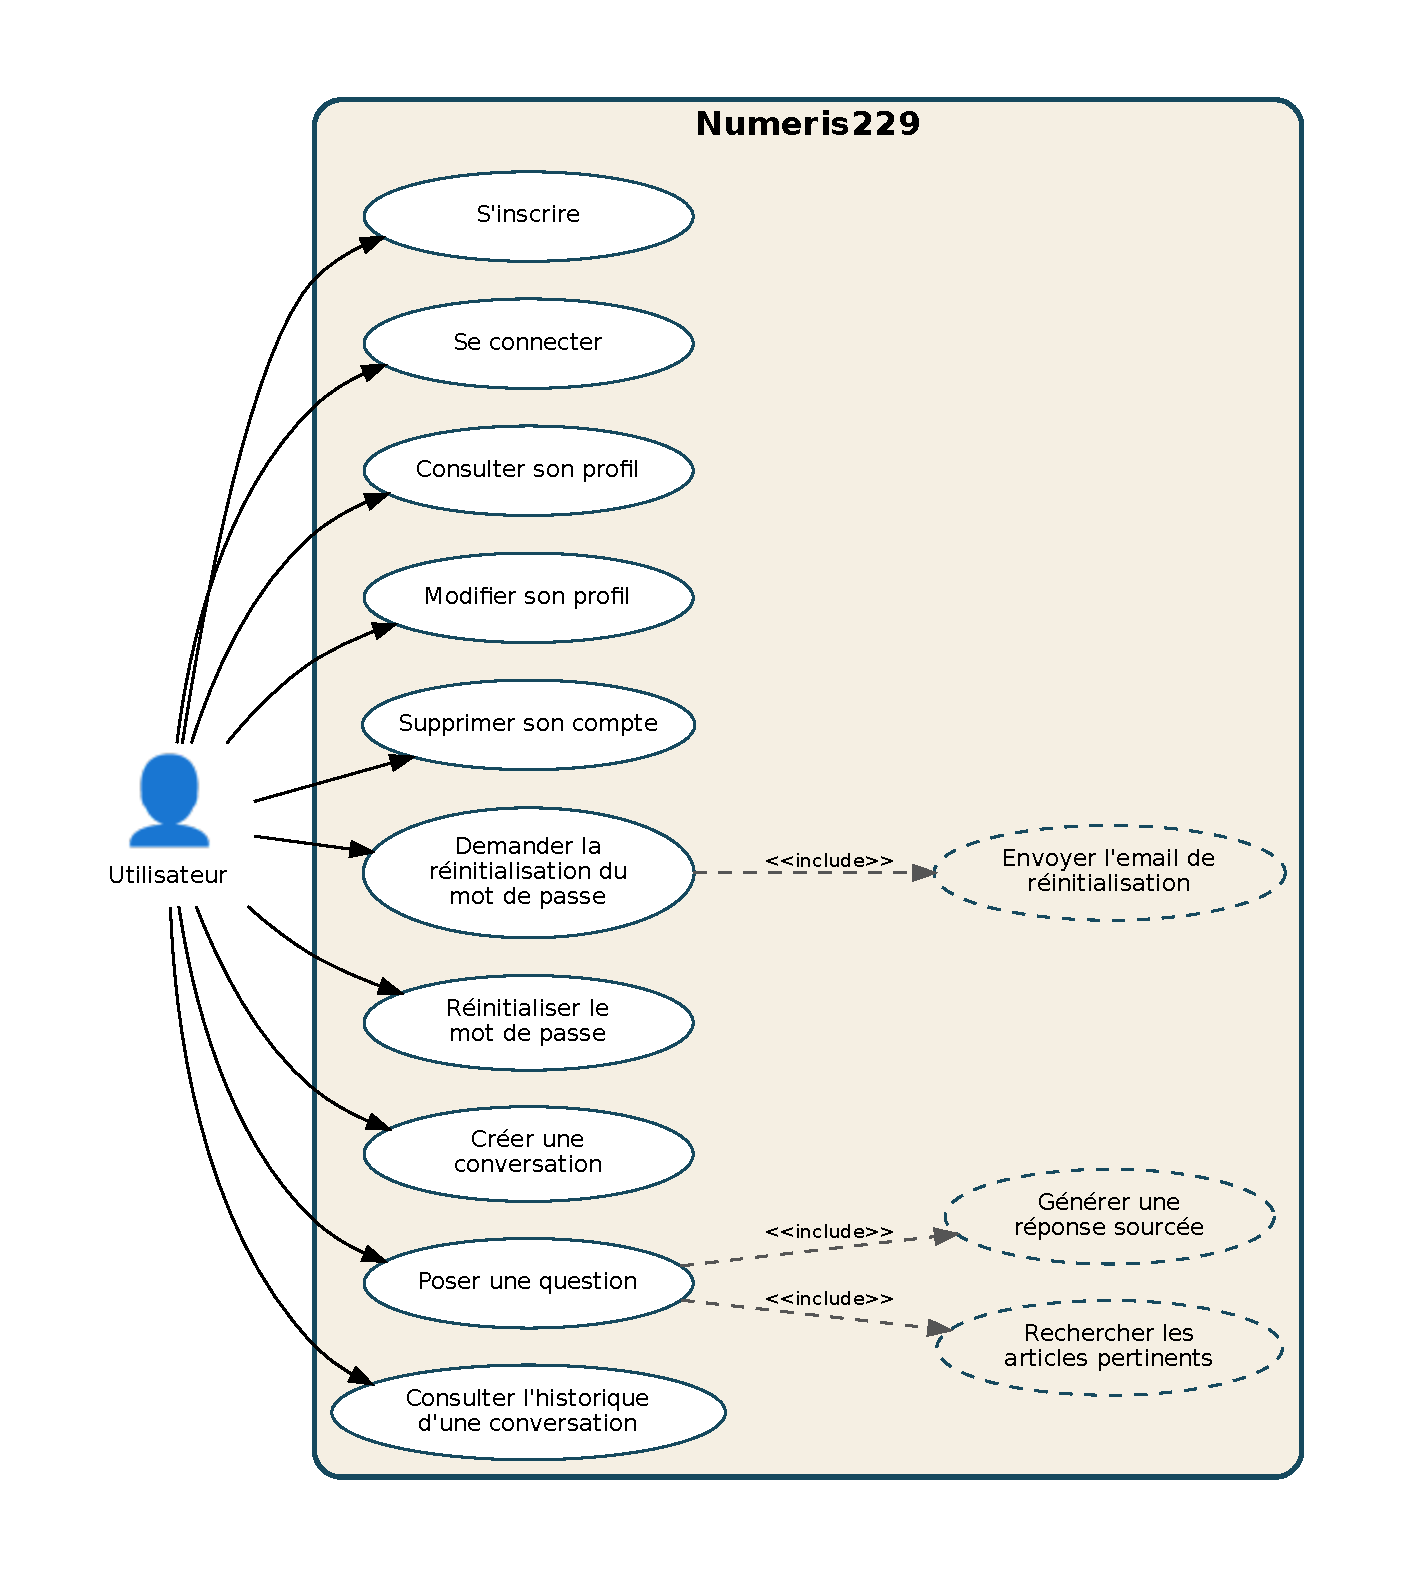
\includegraphics[width=0.85\textwidth]{images/C2/DCU.pdf}
  \caption{Diagramme de cas d'utilisation modélisé sous Visual Paradigm}
  \label{fig:diagramme_cas_utilisation}
\end{figure}

\subsection{Diagramme de classes}

Le diagramme de classes modélisé à la figure \ref{fig:diagramme_classes} expose la structure statique du système, la définition des entités métiers, leurs attributs typés, leurs opérations ainsi que les cardinalités régissant leurs associations.

\subsubsection{Le pôle transactionnel (Espace Utilisateur)}
Ce pôle assure la persistance des interactions au sein de la base de données relationnelle :
\begin{itemize}
    \item \textbf{Classe Utilisateur :} entité maîtresse stockant les informations d'identification (\textit{nom\_prenoms, email, sexe, age, profession, telephone}) et l'empreinte chiffrée (\textit{mot\_de\_passe\_hash}) calculée par hachage salé via l'algorithme bcrypt. Elle encapsule les méthodes de contrôle des identifiants et de purge des données ;
    
    \item \textbf{Classe Conversation :} représente un dossier thématique de consultation. Elle est reliée à la classe \textit{Utilisateur} par une relation de composition forte de multiplicité $1$ vers $0..*$. Cette composition matérialise une dépendance existentielle : une conversation ne peut exister sans son utilisateur propriétaire, et la suppression du compte entraîne automatiquement, par cascade, la suppression de l'ensemble de ses conversations ;
    
    \item \textbf{Classe Message :} constitue l'unité d'échange au sein d'une conversation. Elle conserve la question posée par l'usager, la réponse produite, l'horodatage précis ainsi que la liste des sources juridiques officielles sérialisée au format JSON. Elle est rattachée à la classe \textit{Conversation} par une relation de composition $1$ vers $1..*$.
\end{itemize}

\subsubsection{Le pôle documentaire (Code du Numérique et Chunks RAG)}
Ce pôle modélise la granularité du corpus législatif :
\begin{itemize}
    \item \textbf{Classe Article :} représente chaque disposition unitaire de la Loi N° 2017-20 modifiée. Elle conserve son numéro d'article, son titre, son livre de rattachement, son chapitre ainsi que ses éventuelles mentions de révision législative issues de la Loi N° 2020-35 ;
    
    \item \textbf{Classe ChunkDocumentaire :} matérialise le découpage sémantique d'un article en fragments adaptés aux fenêtres de contexte des modèles d'intelligence artificielle. Chaque chunk est porteur de son texte brut, de son texte enrichi et de ses représentations vectorielles (vecteur dense de dimension 768 et vecteur sparse TF-IDF), permettant le calcul instantané des similarités mathématiques.
\end{itemize}

\begin{figure}[H]
    \centering
    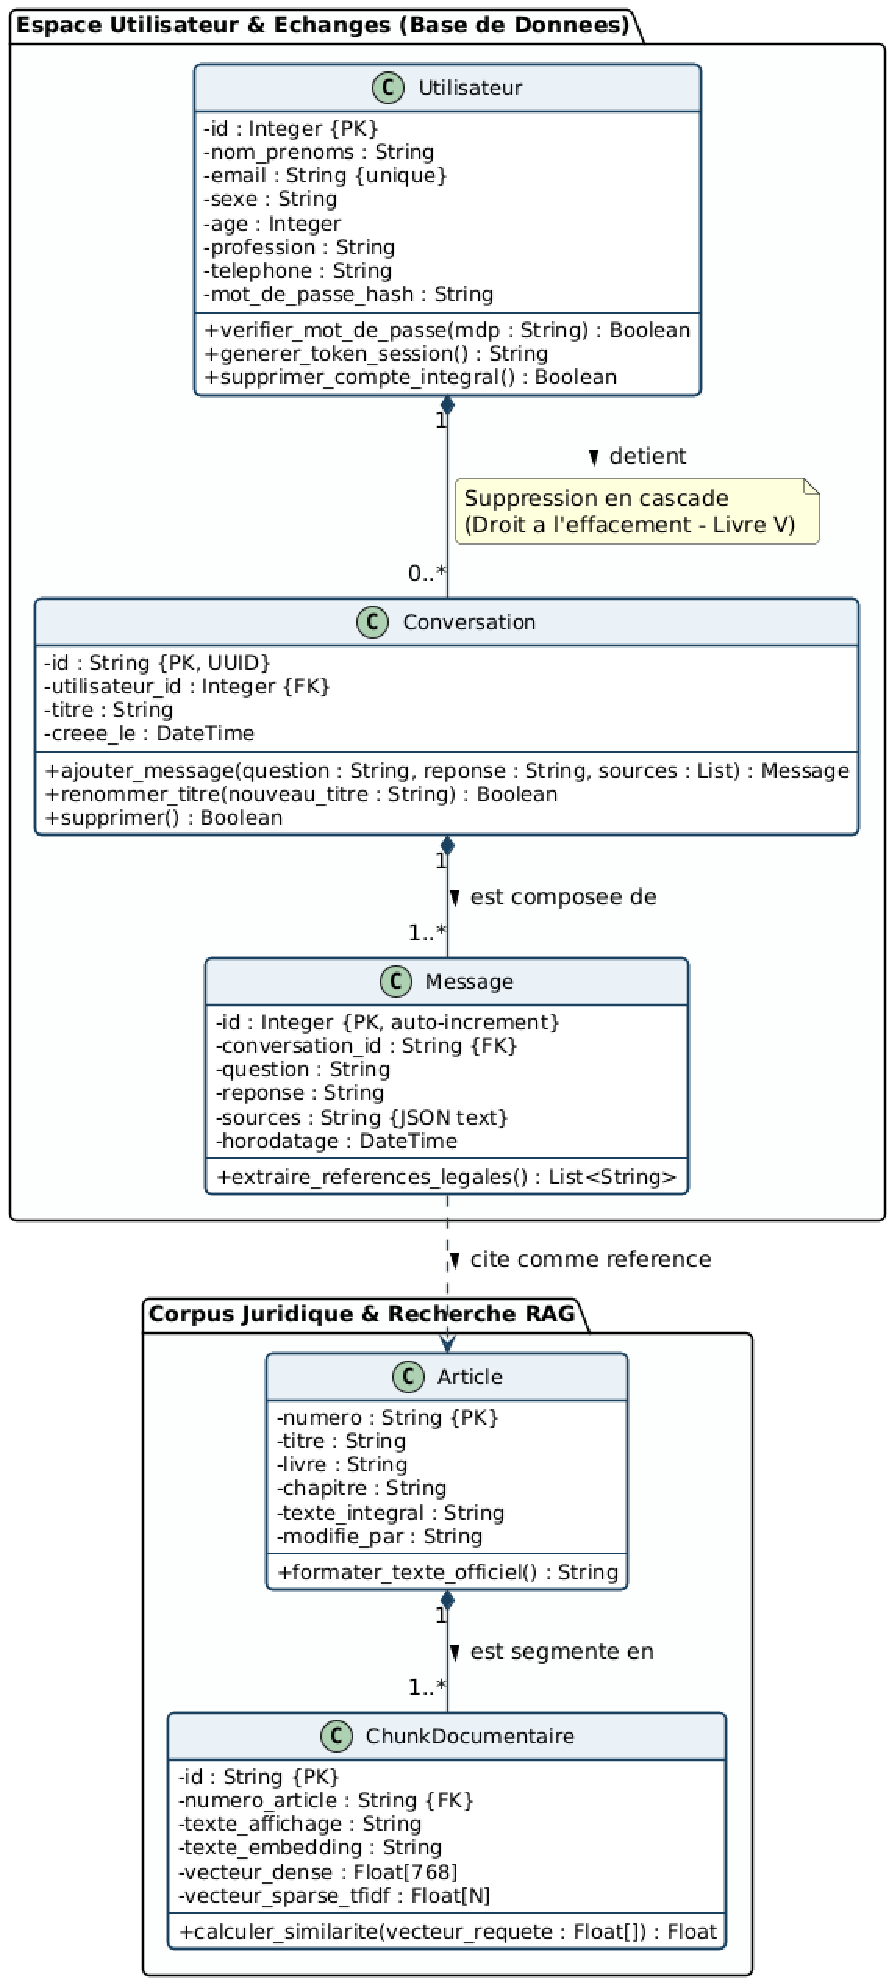
\includegraphics[width=0.95\textwidth]{images/C2/DC.pdf}
    \caption{Diagramme de classes structurel du système Numeris229}
    \label{fig:diagramme_classes}
\end{figure}

\subsection{Diagramme de séquence}

Le diagramme de séquence présenté à la figure \ref{fig:diagramme_sequence} détaille l'enchaînement chronologique des messages et des invocations de méthodes lors du scénario nominal de consultation juridique.

Le cycle de traitement s'articule selon les phases suivantes :
\begin{enumerate}
    \item \textbf{Soumission de la requête :} l'Utilisateur formule sa question en langage naturel sur l'interface Next.js, qui transmet une requête HTTP asynchrone au backend FastAPI en injectant le jeton JWT dans l'en-tête d'autorisation ;
    
    \item \textbf{Vérification d'accès :} le serveur API valide le jeton de session auprès de la base SQLite et transmet la requête à l'orchestrateur \textit{Pipeline RAG} ;
    
    \item \textbf{Routage et recherche documentaire :} l'orchestrateur vérifie si la question contient un numéro formel d'article. En l'absence de numéro explicite, il invoque le \textit{Retriever Hybride} qui calcule simultanément les scores de similarité vectorielle (modèle Solon) et lexicale (modèle TF-IDF) puis extrait les 15 meilleurs chunks candidats ;
    
    \item \textbf{Ré-ordonnancement contextuel :} les 15 candidats sont soumis au modèle \textit{Reranker Cross-Encoder} (CamemBERT) qui opère une évaluation croisée approfondie de chaque extrait vis-à-vis de la question pour ne retenir que les 2 à 3 articles les plus pertinents ;
    
    \item \textbf{Génération souveraine et clause de sauvegarde :} le contexte textuel validé est transmis au serveur local \textit{Ollama} (exécutant le modèle Gemma 3:1B) avec une consigne stricte de citation des articles. Si le serveur d'IA ne répond pas dans le temps imparti (120 secondes), la clause de secours prend immédiatement le relais en extrayant le texte officiel brut sans altération ;
    
    \item \textbf{Persistance et restitution :} le message et ses références légales sont enregistrés en base SQLite, puis retournés au client pour un affichage interactif avec sources dépliables.
\end{enumerate}

\begin{figure}[H]
  \centering
  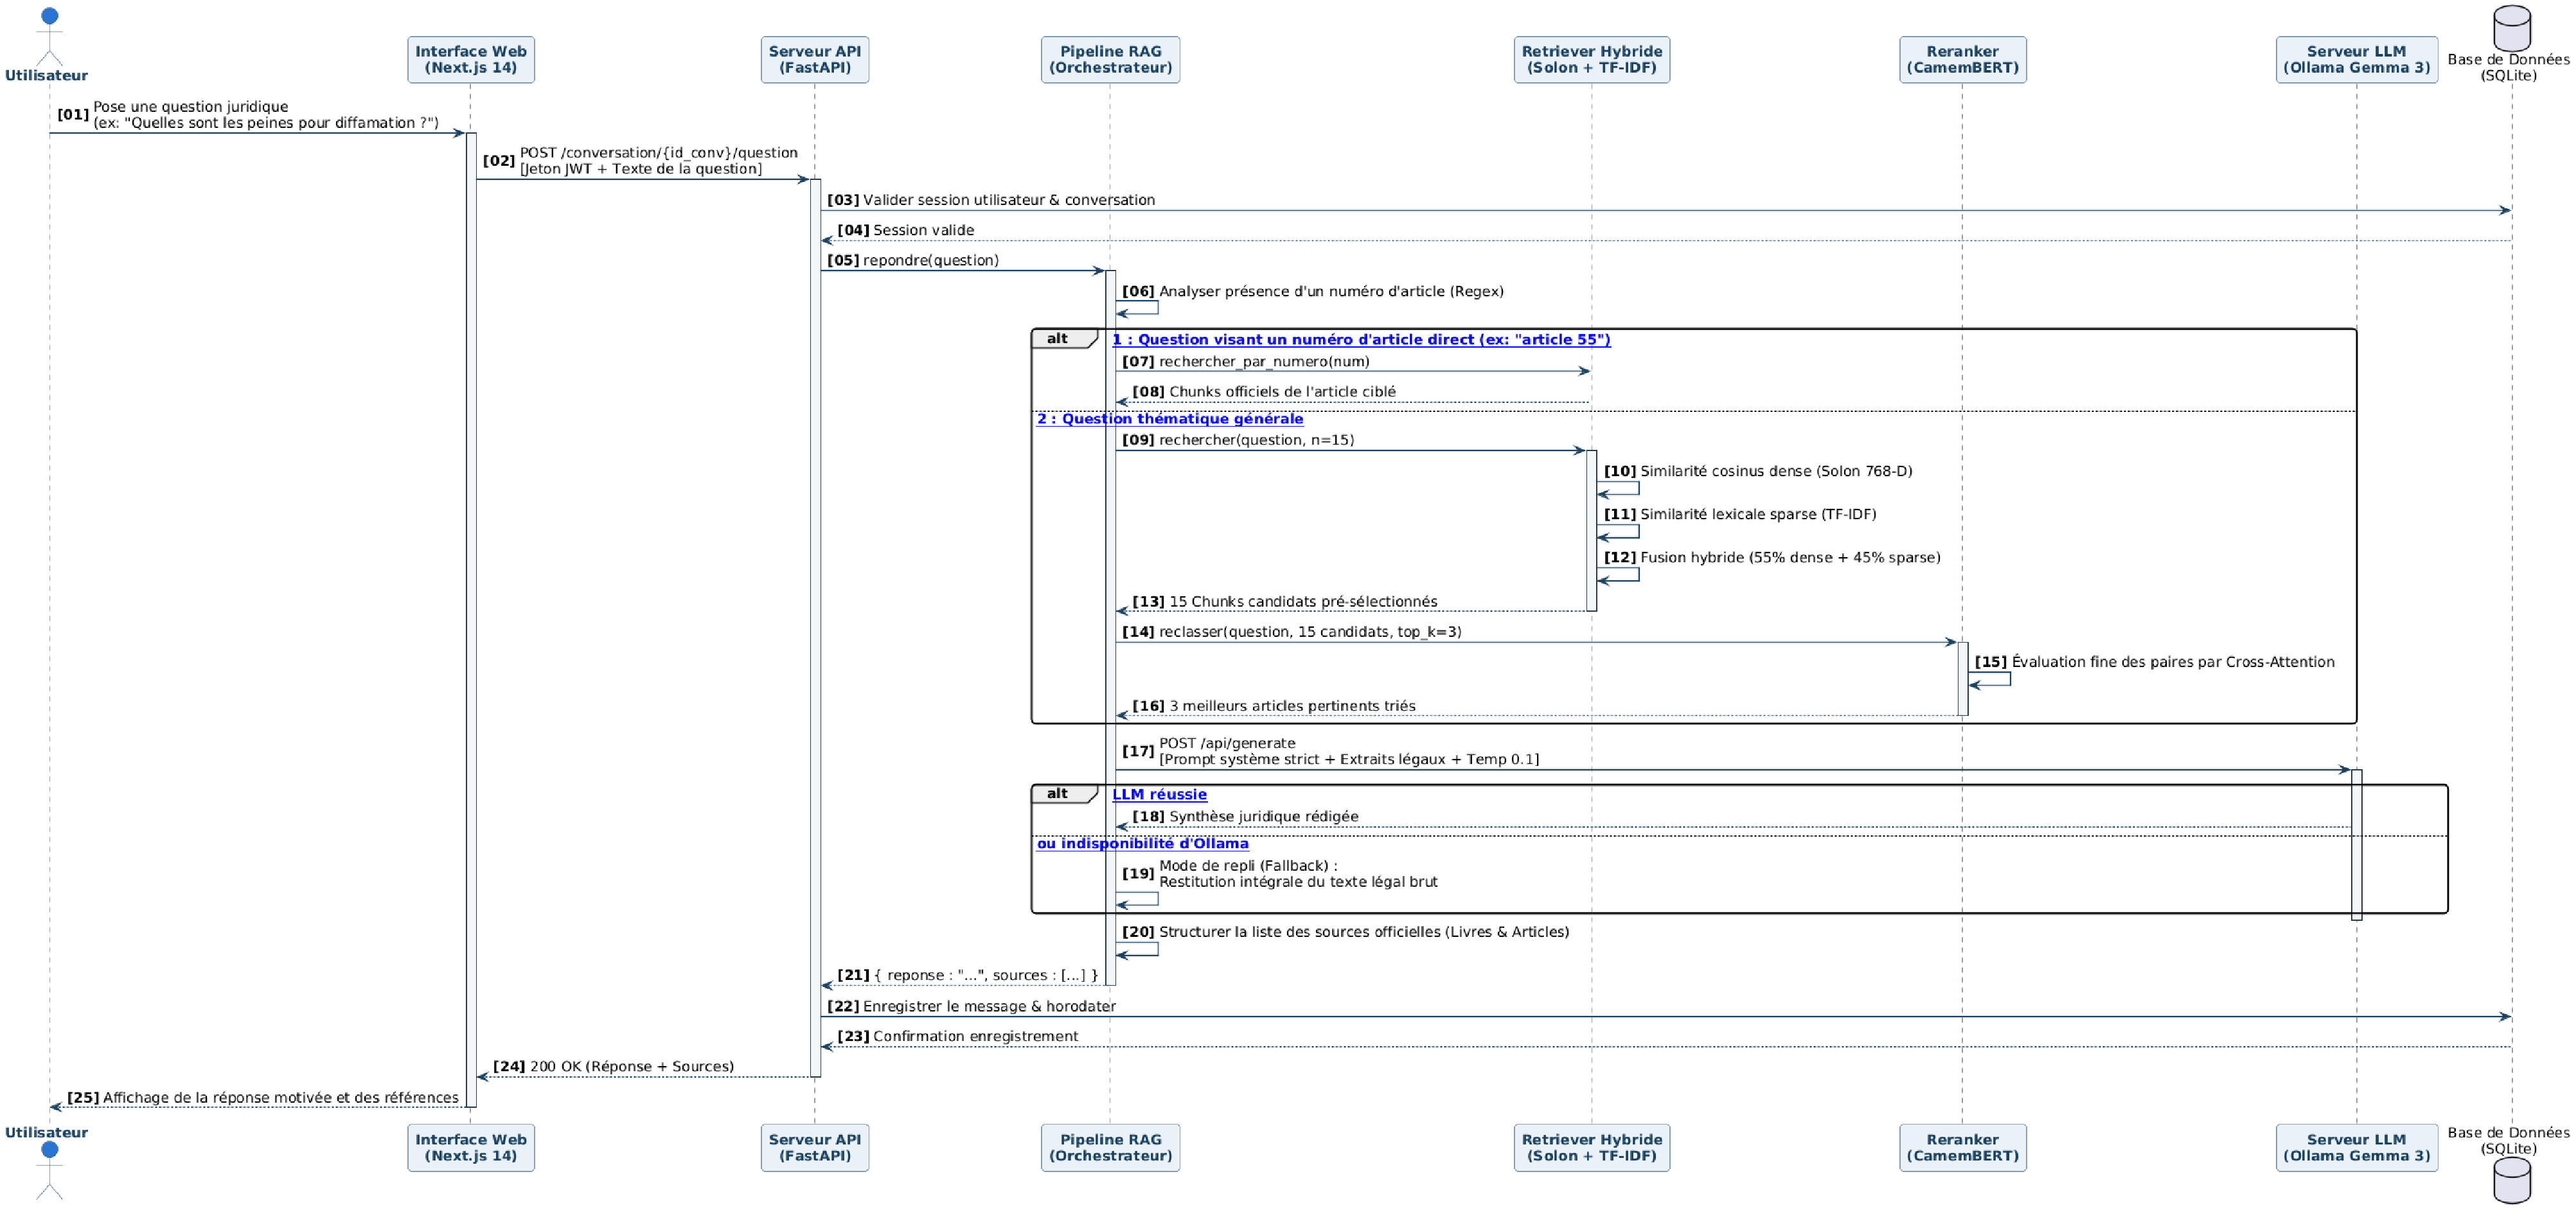
\includegraphics[width=\textwidth]{images/C2/DS.pdf}
  \caption{Diagramme de séquence de la consultation juridique RAG}
  \label{fig:diagramme_sequence}
\end{figure}

\subsection{Diagramme d'activités}

Le diagramme d'activités illustré à la figure \ref{fig:diagramme_activite} cartographie le flux de contrôle opérationnel et les règles de décision conditionnelles appliquées lors de l'exécution d'une requête.

Ce diagramme met en évidence plusieurs mécanismes de sûreté cruciaux :
\begin{itemize}
    \item \textbf{Filtrage d'habilitation initiale :} toute requête émise sans session valide est immédiatement rejetée avec code HTTP 401 et redirection automatique vers l'interface de connexion ;
    
    \item \textbf{Bifurcation selon le type de requête :} le système distingue intelligemment la recherche directe d'article (résolue prioritairement par indexation textuelle exacte) de la recherche thématique sémantique ;
    
    \item \textbf{Parallélisme du Retriever (Fork/Join) :} le calcul dense et le calcul sparse sont exécutés conjointement avant d'être synchronisés pour la normalisation min-max et la fusion pondérée des scores ($55\%$ sémantique / $45\%$ lexical) ;
    
    \item \textbf{Contrôle de pertinence anti-hallucination :} l'algorithme applique une condition de garde stricte sur le score du meilleur candidat ($Score_{max} > -8.0$). Si le sujet n'a aucun fondement dans le Code du Numérique béninois, le système stoppe le pipeline et notifie poliment son incompétence, neutralisant tout risque d'extrapolation trompeuse ;
    
    \item \textbf{Bascule automatique en mode dégradé :} si le modèle de langage subit une défaillance ou un dépassement de délai, le système bascule sans interruption vers la restitution du texte officiel de loi, assurant une disponibilité inaltérable du service.
\end{itemize}

\begin{figure}[H]
    \centering
    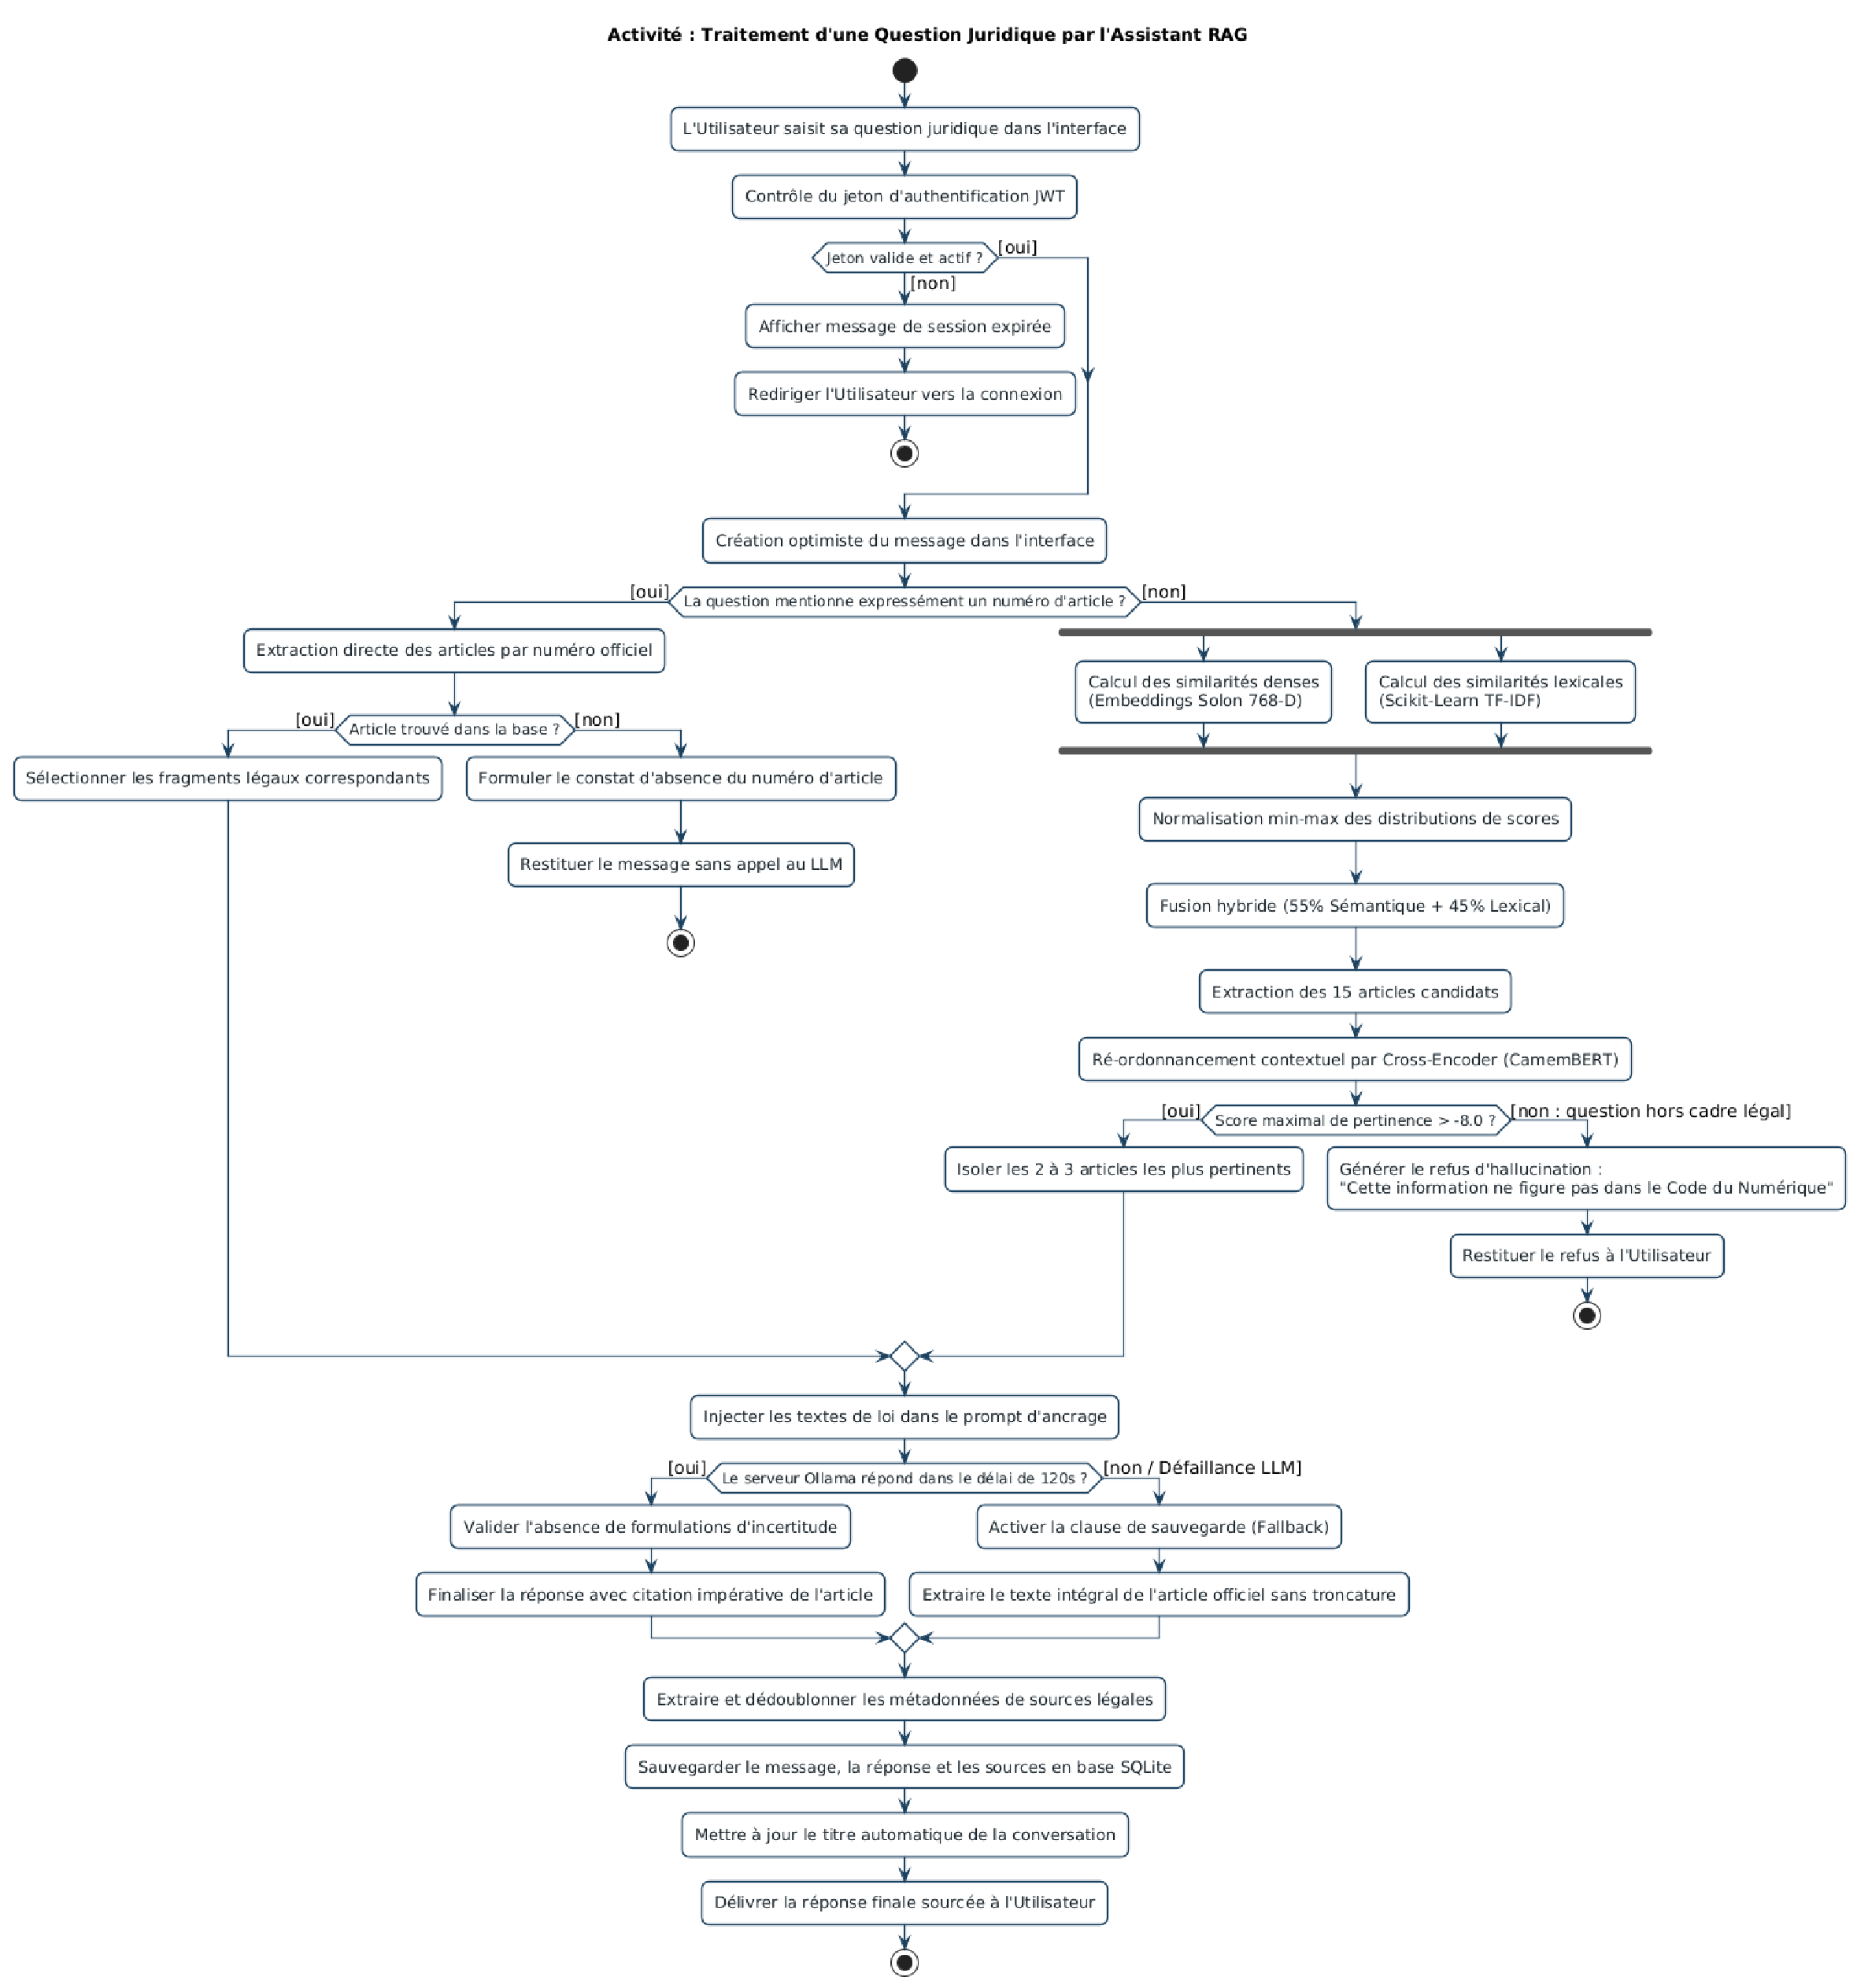
\includegraphics[width=\textwidth]{images/C2/DA.pdf}
    \caption{Diagramme d'activités du processus d'inférence juridique}
    \label{fig:diagramme_activite}
\end{figure}

% ==========================================================
\section{Choix techniques}

\subsection{Justification des technologies utilisées}

Le choix des technologies de \textit{Numeris229} s'appuie sur une analyse multicritères conciliant rigueur scientifique, souveraineté numérique, coût d'infrastructure et conformité aux standards de développement modernes.

\subsubsection{OrdalieTech Solon — modèle d'embeddings juridiques francophones}

La qualité de restitution d'une architecture RAG dépend intimement de la capacité du modèle d'embedding à appréhender les subtilités du vocabulaire juridique. Le modèle retenu est \textbf{OrdalieTech/Solon-embeddings-base-0.1}, un encodeur basé sur SentenceTransformers spécifiquement entraîné sur des corpus juridiques en langue française. Il convertit chaque fragment de texte en un vecteur numérique dense de dimension~768, permettant de capturer les relations sémantiques entre les requêtes profanes et les dispositions normatives du Code du Numérique.

\begin{figure}[H]
    \centering
    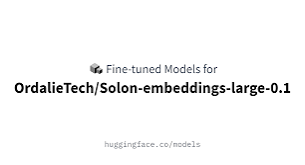
\includegraphics[width=\textwidth]{images/C2/OrdalieTech.png}
    \caption{OrdalieTech Solon}
    \label{fig:ordalietech}
\end{figure}

\subsubsection{Scikit-Learn TF-IDF — recherche lexicale complémentaire}

En matière juridique, la stricte présence d'un terme exact (tel que « diffamation », « signature qualifiée » ou un numéro d'article) est fondamentale. Une recherche purement sémantique peut parfois négliger ces concordances exactes. L'intégration d'un vectoriseur \textbf{TF-IDF} (\textit{Term Frequency - Inverse Document Frequency}) avec analyse des n-grammes $(1, 2)$ permet d'apporter une recherche sparse rapide et précise. La combinaison hybride pondérée ($55\%$ dense Solon et $45\%$ sparse TF-IDF) offre un compromis optimal entre compréhension conceptuelle et exactitude terminologique.

\begin{figure}[H]
    \centering
    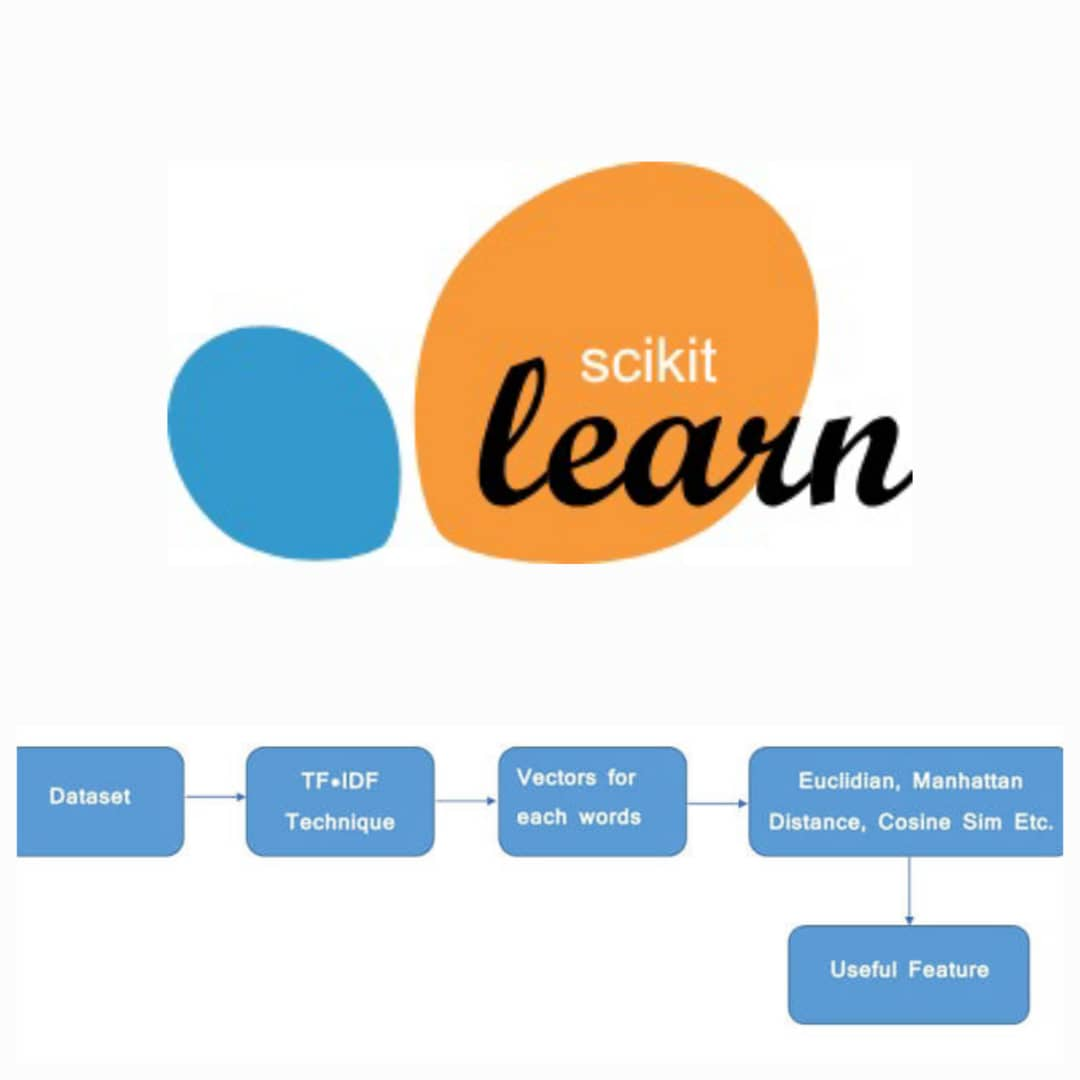
\includegraphics[width=\textwidth]{images/C2/SL-TF IDF.jpeg}
    \caption{Scikit-Learn TF-IDF}
    \label{fig:Scikit-Learn TF-IDF}
\end{figure}

\subsubsection{Cross-Encoder CamemBERT — ré-ordonnancement sémantique (Reranker)}

Pour pallier les limites des modèles bi-encodeurs sur les classements fins, la solution intègre le modèle \textbf{antoinelouis/crossencoder-camembert-base-mmarcoFR}. Contrairement à l'embedding qui traite la question et le document séparément, le cross-encoder évalue la paire question-texte simultanément au moyen de couches d'auto-attention complètes. Il attribue une note de pertinence contextuelle fine à chacun des candidats pré-sélectionnés et permet d'écarter les faux positifs grâce à un seuillage de sécurité strict.

\begin{figure}[H]
    \centering
    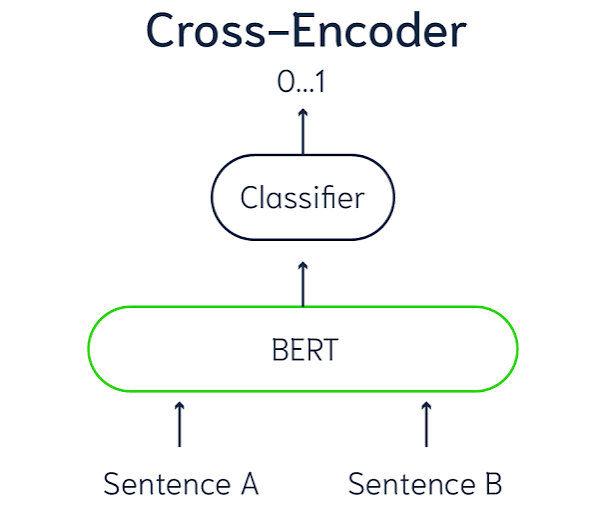
\includegraphics[width=\textwidth]{images/C2/CrossEncoder.png}
    \caption{Schema du reranker}
    \label{fig:reranker}
\end{figure}

\subsubsection{Ollama et Gemma 3 (1B) — modèle de langage local et souverain}

La génération de texte est déléguée au modèle \textbf{gemma3:1b} exécuté localement au travers de la plateforme d'inférence \textbf{Ollama}. Ce choix présente plusieurs bénéfices déterminants :
\begin{itemize}
    \item \textbf{Souveraineté et confidentialité :} aucun transfert de données vers des serveurs tiers hors du territoire national n'est opéré lors de l'analyse juridique ;
    
    \item \textbf{Légèreté et rapidité :} la compacité du modèle (1 milliard de paramètres) autorise une inférence fluide sur CPU tout en garantissant une excellente capacité de reformulation en français ;
    
    \item \textbf{Zéro hallucination :} la configuration d'une température très basse ($0.1$) et d'un prompt d'ancrage juridique strict contraint le modèle à s'appuyer exclusivement sur les articles injectés dans son contexte.
\end{itemize}

\begin{figure}[H]
    \centering
    
\includegraphics[width=\textwidth]{images/C2/Ollama&Gemma.jpeg}
    \caption{Ollama & gemma 3.1}
    \label{fig:Ollama & gemma 3.1}
\end{figure}

\subsubsection{FastAPI et Python — backend API REST asynchrone}

Le backend applicatif est développé en \textbf{Python} avec le framework \textbf{FastAPI}. FastAPI a été sélectionné pour sa rapidité d'exécution asynchrone, son intégration native de \textbf{Pydantic v2} pour la validation stricte des données et la génération automatique de la documentation interactive OpenAPI (Swagger). Python constitue en outre l'écosystème de référence pour l'intégration des bibliothèques de machine learning et de traitement du langage naturel (\textit{SentenceTransformers, Scikit-learn, NumPy}).

\begin{figure}[H]
    \centering
    
\includegraphics[width=\textwidth]{images/C2/Backend.jpeg}
    \caption{Les technologies du Backend}
    \label{fig:Les technologies du Backend}
\end{figure}

\subsubsection{SQLite et SQLAlchemy — base de données transactionnelle}

Pour la persistance des données transactionnelles, le projet s'appuie sur le moteur relationnel \textbf{SQLite} combiné à l'ORM \textbf{SQLAlchemy 2.0}. Ce choix garantit un déploiement autonome, sans dépendance d'infrastructure lourde pour le prototype, tout en assurant une parfaite portabilité et une intégrité relationnelle stricte entre les utilisateurs, les conversations et les messages archivés.

\begin{figure}[H]
    \centering
    
\includegraphics[width=\textwidth]{images/C2/BDOutils.jpeg}
    \caption{La technologie de la base de données}
    \label{fig:Base de données}
\end{figure}

\subsubsection{Next.js 14 et Tailwind CSS — interface web moderne}

Le frontend est réalisé avec le framework \textbf{Next.js 14} (utilisant l'App Router) et \textbf{React 18}. Il offre un rendu performant, une gestion réactive de l'état du chat, ainsi que des routes d'API dédiées au chargement et au cache mémoire des articles du Code du Numérique. L'habillage visuel repose sur \textbf{Tailwind CSS} et les icônes de la suite \textbf{Lucide-React}, offrant une expérience visuelle institutionnelle, claire et adaptée aux directives ergonomiques actuelles.

\begin{figure}[H]
    \centering
    
\includegraphics[width=\textwidth]{images/C2/Frontend.jpeg}
    \caption{Les technologies du frontend}
    \label{fig:Les technologies du frontend}
\end{figure}
\subsubsection{Outils de développement et de modélisation}

L'environnement de travail s'articule autour des outils suivants :
\begin{itemize}
    \item \textbf{Visual Studio Code} en tant qu'environnement de développement intégré (IDE) ;
    \item \textbf{Git et GitHub} pour le versionnement du code source et le suivi collaboratif ;
    \item \textbf{PlantUML} pour la conception et la génération des diagrammes UML normalisés ;
    \item \textbf{LaTeX} pour la rédaction technique et la composition typographique du mémoire.
\end{itemize}

\begin{figure}[H]
    \centering
    
\includegraphics[width=\textwidth]{images/C2/DevOutils.jpeg}
    \caption{Les technologies de développement}
    \label{fig:Les technologies de développement}
\end{figure}

\subsection{Architecture détaillée du système RAG}

Afin d'assurer des consultations juridiques infaillibles, le système \textit{Numeris229} met en œuvre une chaîne RAG (Retrieval-Augmented Generation) structurée en quatre couches interdépendantes :

\subsubsection{Couche d'acquisition et de traitement documentaire}

Cette couche prend en charge le corpus brut de la Loi N° 2017-20 et de sa modification par la Loi N° 2020-35. Les textes légaux ont été nettoyés, structurés par article et découpés en fragments sémantiques (\textit{chunks}). Chaque fragment intègre ses métadonnées descriptives : numéro d'article, titre, Livre de rattachement, mention d'amendement et contexte hiérarchique.

\subsubsection{Couche de recherche hybride (Retriever)}

Lorsqu'une question est soumise, le Retriever procède à une analyse double :
\begin{itemize}
    \item une projection vectorielle dense de la requête calculée par le modèle \textit{Solon-embeddings-base-0.1}, confrontée à la matrice d'embeddings précalculée par similarité cosinus ;
    \item une projection lexicale sparse calculée par \textit{TF-IDF} mesurant la présence de termes et d'expressions clés ;
    \item une normalisation min-max des deux distributions de scores et leur fusion pondérée ($55\%$ sémantique / $45\%$ lexical) pour isoler les 15 articles les plus prometteurs.
\end{itemize}

\subsubsection{Couche de ré-ordonnancement et filtrage (Reranker)}

Les 15 candidats retenus sont transmis au modèle de cross-encoder \textit{CamemBERT mmarcoFR}. Ce dernier évalue chaque couple [requête, extrait légal] et calcule une probabilité fine d'adéquation. Seuls les 2 à 3 meilleurs articles sont conservés. Un seuil critique de score écarte automatiquement les questions non relatives au Code du Numérique afin d'éviter tout traitement illégitime.

\subsubsection{Couche de génération et clause de sauvegarde}

Les extraits légaux validés sont injectés dans un template de prompt institutionnel instruisant le modèle de langage \textit{Gemma 3} de formuler une réponse synthétique et explicite en français formel, avec obligation de mentionner les articles de référence. Si le serveur d'inférence ne répond pas dans le délai imparti, une routine de sauvegarde extrait le texte complet de l'article officiel le plus pertinent et le restitue intégralement à l'utilisateur, assurant une disponibilité ininterrompue de l'information juridique.

\subsection{Choix du déploiement}

La stratégie de déploiement de \textit{Numeris229} privilégie la modularité et la souveraineté :

\begin{itemize}
    \item \textbf{Frontend web :} l'application Next.js 14 peut être hébergée sur des plateformes de bordure cloud telles que Vercel, bénéficiant d'un réseau mondial de distribution de contenu (CDN) et d'un temps d'affichage optimal pour les utilisateurs béninois et internationaux ;
    
    \item \textbf{Serveur d'API et inférence IA :} le backend FastAPI et le moteur d'inférence Ollama sont conçus pour être déployés sur un serveur privé virtuel (VPS) dédié ou au sein d'une infrastructure cloud souveraine (conteneurs Docker). Cette approche garantit le contrôle intégral des modèles d'IA, l'absence de fuite de données vers des services tiers et la maîtrise des coûts opérationnels ;
    
    \item \textbf{Persistance des données :} la base SQLite locale assure une administration simplifiée lors des phases de développement et d'évaluation, avec la possibilité d'une migration transparente vers PostgreSQL lors du passage à une échelle de production institutionnelle.
\end{itemize}

% ==========================================================
\clearpage
\section*{Conclusion}
\addcontentsline{toc}{section}{Conclusion}

Ce chapitre a présenté l'analyse des besoins, la conception détaillée ainsi que les choix technologiques retenus pour la réalisation de \textit{Numeris229}. La formalisation des besoins fonctionnels et non fonctionnels a mis en lumière la nécessité d'une plateforme alliant accessibilité pour le citoyen et rigueur pour le professionnel du droit. Les diagrammes UML élaborés ont permis d'établir une cartographie précise des interactions, de la structure des données et des flux d'exécution. Enfin, la combinaison innovante d'une recherche hybride (Solon dense et TF-IDF sparse), d'un ré-ordonnancement par cross-encoder CamemBERT et d'une inférence souveraine sous Ollama confère à la solution une fiabilité optimale sans risque d'hallucination. Ces fondations techniques et conceptuelles introduisent l'implémentation et les résultats expérimentaux détaillés dans le chapitre suivant.
